%%%% ijcai18.tex

\typeout{Galaxy Network Embedding: A Hierarchical Community Structure Preserving Approach}

% These are the instructions for authors for IJCAI-18.
% They are the same as the ones for IJCAI-11 with superficical wording
%   changes only.

\documentclass{article}
\pdfpagewidth=8.5in
\pdfpageheight=11in
% The file ijcai18.sty is the style file for IJCAI-18 (same as ijcai08.sty).
\usepackage{ijcai18}

% Use the postscript times font!
\usepackage{times}
\usepackage{xcolor}
\usepackage{soul}
\usepackage[utf8]{inputenc}
\usepackage[small]{caption}

% wy add
\usepackage{helvet}  %Required
\usepackage{courier}  %Required
\usepackage{url}  %Required
\usepackage{graphicx}  %Required
\usepackage{algorithm}
\usepackage{algorithmicx}
\usepackage[noend]{algpseudocode}
\usepackage{amsmath}

\usepackage{subfigure}

\usepackage{CJK}
\usepackage{array}
\usepackage{amsthm}
\usepackage{amssymb}

\theoremstyle{definition}
\newtheorem{defn}{Definition}


\renewcommand{\algorithmicrequire}{\textbf{Input:}} % Use Input in the format of Algorithm
\renewcommand{\algorithmicensure}{\textbf{Output:}} % Use Output in the format of Algorithm

%TODO PACKAGE, DELETE THEM ALL!!
\usepackage{lipsum}                     % Dummytext
\usepackage{xargs}                      % Use more than one optional parameter in a new commands
%\usepackage[pdftex,dvipsnames]{xcolor}  % Coloured text etc.
% 
\usepackage[colorinlistoftodos,prependcaption,textsize=tiny]{todonotes}
\newcommandx{\unfinished}[2][1=]{\todo[linecolor=red,backgroundcolor=red!25,bordercolor=red,#1]{#2}}
\newcommandx{\change}[2][1=]{\todo[linecolor=blue,backgroundcolor=blue!25,bordercolor=blue,#1]{#2}}
\newcommandx{\info}[2][1=]{\todo[linecolor=OliveGreen,backgroundcolor=OliveGreen!25,bordercolor=OliveGreen,#1]{#2}}
\newcommandx{\improvement}[2][1=]{\todo[linecolor=Plum,backgroundcolor=Plum!25,bordercolor=Plum,#1]{#2}}
\newcommandx{\thiswillnotshow}[2][1=]{\todo[disable,#1]{#2}}
\newcommand{\origin}[1]{{\color{blue}{#1}}}
\newcommand{\new}[1]{{\color{red}{#1}}}


% the following package is optional:
%\usepackage{latexsym} 

% Following comment is from ijcai97-submit.tex:
% The preparation of these files was supported by Schlumberger Palo Alto
% Research, AT\&T Bell Laboratories, and Morgan Kaufmann Publishers.
% Shirley Jowell, of Morgan Kaufmann Publishers, and Peter F.
% Patel-Schneider, of AT\&T Bell Laboratories collaborated on their
% preparation.

% These instructions can be modified and used in other conferences as long
% as credit to the authors and supporting agencies is retained, this notice
% is not changed, and further modification or reuse is not restricted.
% Neither Shirley Jowell nor Peter F. Patel-Schneider can be listed as
% contacts for providing assistance without their prior permission.

% To use for other conferences, change references to files and the
% conference appropriate and use other authors, contacts, publishers, and
% organizations.
% Also change the deadline and address for returning papers and the length and
% page charge instructions.
% Put where the files are available in the appropriate places.

\title{Galaxy Network Embedding: A Hierarchical Community Structure Preserving Approach}

% Single author syntax
\author{Jêröme Lang\\ 
Laboratoire d'Analyse et Modélisation des Systèmes pour l'Aide à la Décision (LAMSADE)  \\
pcchair@ijcai-18.org}

% Multiple author syntax (remove the single-author syntax above and the \iffalse ... \fi here)
\iffalse
\author{
First Author$^1$, 
Second Author$^2$, 
Third Author$^3$, 
\\ 
$^1$ First Affiliation \\
$^2$ Second Affiliation\\
$^3$ Third Affiliation  \\
%
first@email.address,
second@email.address,
third@email.address
}
% If your authors do not fit in the default space, you can increase it 
% by uncommenting the following (adjust the "2.5in" size to make it fit
% properly)
% \setlength\titlebox{2.5in}
\fi

\begin{document}

\maketitle

\begin{abstract}
	Network Embedding is a method to learn the low-dimensional vector representations of nodes under the condition of preserving different kinds of the network properties. Previous researches mainly focus on preserving nodes' attributes, neighborhood information, or community structure on a particular resolution, but can not preserve the hierarchical community structure which enables that the network can be easily analyzed on various resolutions. In this paper, we formulate a constrained optimization problem to describe the hierarchical community structure preserving network embedding and propose the Galaxy Network Embedding (GNE) model to solve the problem. The representations of nodes reflect the hierarchical community structure with the spherical galaxy model. In detail, we present an approach to embed communities into an $m$-dimensional spherical surface whose center represents the parent community they belong to. The experiments on Hierarchical Random Graphs and real networks reveal that the GNE preserves the hierarchical community structure integrally and shows advantages in several applications such as multi-classification and network visualization. The source code of GNE is available online.

\end{abstract}

\section{Introduction}

Complex network, an abstraction and analytical means of the complex system, has been widely used in multidisciplinary fields. 
		The analysis for complex networks becomes increasingly significant. However, the traditional network representation induces the sparsity issue (such as adjacency matrix) \cite{Perozzi2014DeepWalk}.
		Network embedding is an approach to learn the low-dimensional representation of complex network vertices by neural network \cite{Grover2016node2vec} or matrix decomposition \cite{Wang2017Community} under the condition of preserving different kinds of the structure information of the network. Through the network embedding, many general machine learning methods can be applied for fast and effective vertices classification, clustering and network visualization \cite{bhagat2011node} \cite{yan2007graph}.
		
		Previous network embedding methods mainly focus on preserving the local neighborhood structure and the attributes of vertices, e.g. Isomap \cite{Tenenbaum2000A} preserves the first-order proximity between vertices; \cite{Tang2015LINE} and \cite{Wang2016Structural} consider the second-order proximity; \cite{Cao2015GraRep} extends to preserve high-order proximity.  
		
		Recently, \cite{Wang2017Community} propose a Modularized Nonnegative Matrix Factorization(MNMF) model for community preserving network embedding, which considers both the microscopic structure and the mesoscopic community structure. They define a similarity matrix to describe the microscopic structure and utilize the community indicator matrix obtained by community detection to describe the mesoscopic structure. The embedded vectors are obtained by decomposing the two matrices, similar with \cite{Yang2015Network}.
        
		These methods only utilize the neighborhood information of the vertices or the community detection information on a particular resolution, but can not completely preserve all the community structure information of the network. Actually, if observed at different resolutions, a network can be divided into communities on different resolutions. Such a hierarchical community structure can be described as a tree structure (see Figure \ref{fig:intuition}. (a) (b)). For instance, a person in the social network can be seen as coming from a city, a state or a country. Thus, a network embedding method with hierarchical community preserved is required. In the case above, we expect to attain the users' social relationships at the city level, state level, and country level simultaneously with only one training process. In a word, compared with the classical embedding methods, the hierarchical community preserving network embedding can provide richer structural information, and make it easier to analyze the network on different resolutions.

		It is challengeable to formulate the hierarchical community preserving network embedding. 
		We interpret the essence of the hierarchical community structure from two perspectives. 
		Horizontally, the nodes in the same community are more similar to each other. Vertically, a community in the deeper level has a greater cohesion degree. Besides defining an optimization problem with constraints above, it is also a challenge to solve the problem effectively and efficiently.

		In this paper, we define a constrained optimization problem to formulate the hierarchical community structure preserving network embedding and propose the Galaxy Network Embedding (GNE) model to solve it. We regard communities composed of sub-communities as galaxies, another type of systems with hierarchical structure, composed of stellar systems (see Figure \ref{fig:intuition}. (b) (c)). Inspired by the galaxy structure, we embed sub-communities on an $m$-dimensional spherical surface whose spherical center is the parent community they belong to. The radii of the embedded communities indicate the cohesion degree. The embedding process of all communities and vertices is recursively implemented as described above.
		
		To summarize, we make the following contributions:
		\begin{itemize}
		\item{
		We formulate the hierarchical community structure preserved network embedding as an optimization problem with constraints and present a novel method to transform the difficult optimization problem into an unconstrained optimization problem more easily to be solved.
		}
		\item{
		We propose the Galaxy Network Embedding (GNE) model based on a novel spherical embedding method, which preserves the hierarchical community structure on any resolution while embedding the vertices or communities of a network into low-dimensional vectors in Euclidean space.
		}
		\item{
		GNE is extensively evaluated on four real networks and four synthetic networks. The experiment results demonstrate that our model can integrally preserve the hierarchical community structure and is significantly superior to other models on vertex classification and network visulization.  
		}
		\end{itemize}
		
		
		\begin{figure}
			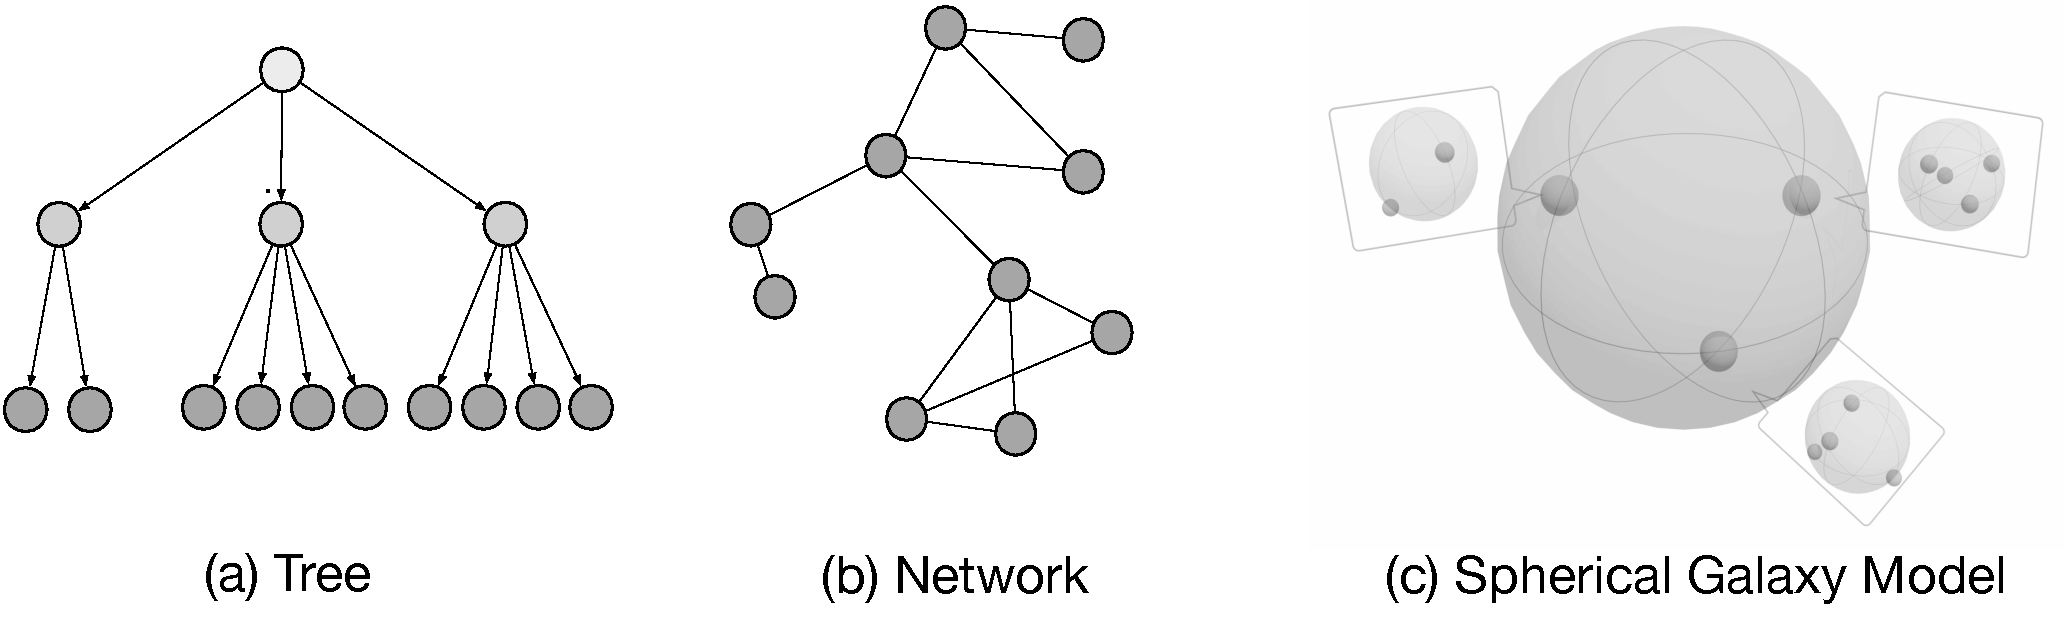
\includegraphics[width=1.0\linewidth]{figure/Galaxy.pdf}
			\caption{Different display approaches of the network hierarchical structure.}
			\label{fig:intuition}
		\end{figure}

\section{Related Work}
	
	\subsection{Network Embedding}
	Network embedding maps the vertices or edges of a network into a low-dimensional vector space, which is beneficial at vertex classification and network visualization. Lots of excellent works are developed on learning the network representation. DeepWalk \cite{Perozzi2014DeepWalk} reveals that the distribution of vertices appearing in short random walk follows a power-law, similar with the distribution of words in natural languages. Thus, it combines truncated random walk \cite{fouss2007random-walk} with the Skip-Gram \cite{mikolov2013efficient} to learn vertex representations. 
	Compared with DeepWalk, Node2Vec \cite{Grover2016node2vec} designs a kind of flexible network neighbourhood sampling strategy and proposes a biased random walk to learn vertex representations with Skip-Gram. LINE \cite{Tang2015LINE} formulates a novel optimization problem based on first- and second-order proximity on network embedding. Compared with LINE, GraRep \cite{Cao2015GraRep} integrate the $k$-step information to learn vertex representations. MNMF \cite{Wang2017Community} considers that community, as a mesoscopic description of the network, plays an important role in the network representation. Thus, it incorporates the community structure into network embedding. All the methods above mainly focus on preserving the pairwise proximity or community structure on a particular resolution, however, the community structure on different resolutions are not considered. 

	\subsection{Hierarchical Network}
	Actually, many complex networks in the real world have hierarchical community structure.
	\cite{newman2003structure} introduces the community structure of the network, and summarizes that complex networks have the small-world property and the scale-free property. \cite{song2005self} finds that a large number of real networks have the self-similar property, i.e. a part of a network is similar with the whole network to some extent. 
	\cite{clauset2008hierarchical} uses hierarchical random graph, similar in spirit to the tree-based models used in some studies of network search and navigation, to model this kind of hierarchical community structure and generate the hierarchical network.
	In the hierarchical random graph, the probability of an edge appearing between two vertices depends on the level that their nearest common ancestor locates in. 
	Embedding the hierarchical community structure into low-dimensional vector spaces has not been investigated yet.

	\section{Problem Definition}
		We formally define the problem of hierarchical structure preserving network embedding and introduce the optimization objective of the problem. 
	
		We first give the definition of the hierarchical clustering tree \cite{clauset2008hierarchical} of a network.
		\begin{defn}[\textbf{\emph{Hierarchical Clustering Tree of Network}}]
			Given an undirected network $G = (V, E)$, the hierarchical clustering tree of $G$ is denoted as $T$ with a depth of $L$, where $V$ represents the vertex set and $E$ represents the edge set of $G$. We denote $C$ as the node set,
			% as well as the community set of $G$. 
			$C^l$ as the node set at the $l$-th level and $c^l_i$ as the $i$-th node at the $l$-th level of $T$. $\Gamma(c)$ denotes the child node set of the node $c$ and $\delta(c)$ denotes the parent node of $c$. Meanwhile, $c^l_i$ also represents the $i$-th community while recursively dividing $G$ at the $l$-th level. For the $l$-th level of $T$,
				\[
				\forall c^l_i, c^l_j \in C^l \quad c^l_i \cap c^l_j = \varnothing
				\]
				\[
				\bigcup_i c_i^l = V.
				\]
			Especially, $c_1^1$ is the root node of $T$ and also the node set of $G$ (i.e. $c_1^1 = V$) and $c_i^L = \{v_i\}$, where $v_i$ is the $i$-th vertex of the $G$.
		\end{defn}
			%For brevity, we use $T$ to denote $T_G$. The notations of the variables used in the following paragraph are given here:  
		
	 
		
		In order to preserve the hierarchical structure property of the network explicitly, we embed not only the vertices but also the communities of all levels. Therefore, our model can preserve the structure property on all resolutions. As a community of $G$, the leaf node $c_i^L$ contains only one vertex $v_i$, thus the representation of $v_i$ is equivalent to $c_i^L$. For brevity, we use community representation instead of vertex representation in the model. We define the community representation:
		\begin{defn}[\textbf{\emph{Community Representation}}]
			Given a network $G$ and its hierarchical clustering tree $T_G$, the community representation is a function $\Phi: C \rightarrow R^m$ ($m \ll |C|$) which can preserve the structure property of $G$.
		\end{defn} 
	    In our scenario, we hope that the community representation can preserve two kinds of properties of $G$. One is the local information, \new{ i.e. the pairwise proximity between sub-communities in the same community.} \origin{(i.e. the pairwise proximity between the child nodes deriving from the same parent node in $T$)}. The other is the hierarchical structure property, i.e. the parent-child relationship and siblings relationship contained in the tree structure. The formalized definition of the two properties will be given in the following paragraph. 
	    
	    
	    In order to preserve the local information between communities, we introduce the community proximity extended from the definition of the common neighbour similarity \cite{libennowell2007the}:
		\begin{defn}[\textbf{\emph{Community Proximity}}]
			Community proximity is the pairwise similarity between communities in a network. It can be calculated according to the average similarity of the members belonging to different communities. Based on common neighbour similarity, We define the proximity between $c^l_i$ and $c^l_j$.
			\begin{equation}
			S_{i,j}^k = \frac{1}{|c_i^l||c_j^l|}\sum_{u \in c_i^l} \sum_{v \in c_j^l} \xi_{u, v}
			\end{equation} 
			where $c_i^l, c_j^l \in \Gamma(c_k^{l-1})$
			and $\xi_{u, v}$ is the similarity between the vertex pair $u$ and $v$ shown as follows :
			\begin{equation}
			\xi_{u,v} = \frac{A_u^TA_v}{\sqrt{||A_u||_1||A_v||_1}},
			\end{equation}
			where $A$ is the adjacency matrix of $G$, $A_u$ is the $u$-th column of the $A$.
			
		\end{defn}
		Taking community proximity preservation into consideration, we can set up the optimization objective. The concrete form can be defined referring to many traditional researches \cite{Tang2015LINE} \cite{mikolov2013efficient}. In this paper, we extend the 1-step optimization objective in GraRep \cite{Cao2015GraRep}. To preserve the proximity between communities deriving from the same parent node $c_k^{l-1}$, the objective is defined as: 
		\begin{equation}
		\label{equ:local_loss} 
		\begin{split}
		O^{(k)}(\Phi, \Phi') & = \sum_{c_i^l, c_j^l \in \Gamma(c_k^{l-1})} \frac{S_{i,j}^l}{\sum_t S_{i, t}^l} \cdot \log{\sigma(\Phi(c_i^l)^T \Phi'(c_j^l))} \\
		+ \frac{\lambda}{|\Gamma(c_k^{l-1})|}&\sum_{c_e^l \in \Gamma(c_k^{l-1})} \frac{S_{i, e}^l}{\sum_t S_{i, t}^l} \cdot \log{\sigma(-\Phi(c_i^l)^T \Phi'(c_e^l))}, \\
		\end{split}
		\end{equation}
		where $\sigma(\cdot)$ is the sigmoid function defined as $\sigma(x) = (1+e^{-x})^{-1}$, $\lambda$ is a hyper-parameter related to negtive sampling indicating the number of negative samples, $\Phi(c)$ is the "current" vector \cite{Cao2015GraRep} of community $c$ we want and $\Phi'(c)$ is the "context" vector \cite{Cao2015GraRep} of community $c$ which is an auxiliary variable.  

		
		In order to preserve hierarchical structure properties, we impose constraints on the embedded communities, which can make the optimization objective more intuitive and the model more explainable. The constraints can be divided into two aspects: horizontal and vertical. Horizontally, vertices belonging to the same community should be closer to each other than those belonging to different communities (i.e. their intra-cluster similarities are higher). Therefore, we suppose that the Euclidean distance between sub-communities belonging to the same community should be less (see the first constraint of Eq. \ref{equ:whole_loss}). Vertically, as the division granularity decreases, the cohesion degree of communities will increase. That means the cohesion degree of low level communities should be less than that of high level ones in $T$. Reflecting the property into Euclidean space, we have the second constraint of Eq. \ref{equ:whole_loss}.
		We give the detailed definition of Hierarchical Preserving Network Embedding: 
		\begin{defn}[\textbf{\emph{Hierarchical Preserving Network Embedding}}]
			The Hierarchical Preserving Network Embedding problem is formally defined as a constrained optimization problem:
			\begin{equation}
			\label{equ:whole_loss}
			\begin{split}
			\min_{\Phi,\Phi'} & \sum_l^{L-1}\sum_{c^k_l \in C^l} O^{(k)}(\Phi, \Phi') \\
			s.t. \quad
			|| \Phi(c_u^l) - & \Phi(c_v^l) || - ||\Phi(c_u^l) - \Phi(c_w^l)|| < 0, \\
			|| \Phi(c_i^{l+1}) - & \Phi(c_j^{l})) || - ||\Phi(c_j^{l}) - \Phi(c_k^{l - 1})|| < 0,\\
			\end{split}
			\end{equation}
			where,
			\[
			\begin{split}
				\delta(c_u^l) = \delta(c_v^l), \quad \delta(c_u^l) \neq \delta(c_w^l)\\
				\delta(c_i^{l+1}) = c^l_j, \quad \delta(c^l_j) = c^{l - 1}_k \\ 
			\end{split}
			\]
		\end{defn}
	It can be seen that the constrained optimization objective Eq. \ref{equ:whole_loss} is very complex, the number of whose constraints reaches $O (|V|^3) $. It is hard to solve the optimization problem directly. In the later section, we simplify the problem by imposing stronger constraints.
	
	\section{Galaxy Network Embedding Model}
	\label{sec:model}
	Inspired by the structure of galaxies in the real world, we propose the GNE model to solve the optimization problem above efficiently through imposing more constraints.  
	 \subsection {Overview}
	 \subsubsection{Properties of Galaxy Structure}
	 \begin{figure}
		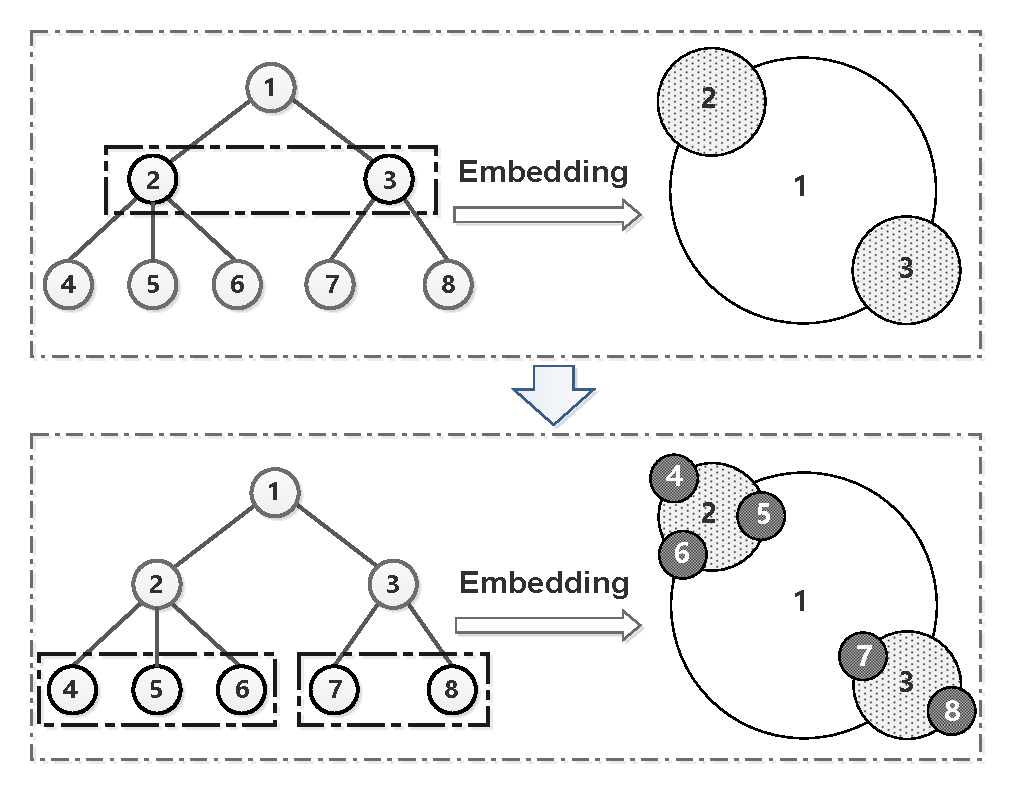
\includegraphics[width=1\linewidth]{figure/Structure.pdf}
		\caption{Structure of GNE}
		\label{fig:structure}
	\end{figure}
	 As well known, Galaxy structure has the similar hierarchical property (see Figure \ref{fig:structure}). For example, the Galaxy includes many stellar systems such as the solar system, while the solar system also consists of several planets. In order to express conveniently, we assume that a galaxy has spherical structure with radius $r_i$ and the center located at $x_i$. The galaxy structure satisfies that the distance between two galaxies is much larger than the radius of each of them, namely, 
	 
	 \begin{equation}
	 	  r_i, r_j \ll ||x_i - x_j||_2 
	 \end{equation}
	 It is evident that if the distribution of the embedded communities is consistent with the structure of galaxies, the constraints of Eq. \ref{equ:whole_loss} can be satisfied. Therefore, we introduce the galaxy structure into our model. 
	 \subsubsection{Model Framework based on Galaxy Structure}
	 First, we simplify the Galaxy model. \origin{We suppose that the distances from each galaxy to the center of its galaxy group are equal. In other words, all galaxies are located at a spherical surface.} \new{We suppose that galaxies are located at a spherical surface. In other words, the distances from each galaxy to the center of its galaxy group are equal.} Specifically, besides the Euclidean representation $\Phi(c_i^l)$, each embedded community $c_i^l$ has another attribute $r_i^l$ (the radius of the corresponding galaxy group). We have the following constraints:
	 \begin{equation}
	 \label{equ:sphere_constraints}
	 \begin{split}
	 	\forall c_i^{l+1} & \in \Gamma(c_k^l), \quad l = 1, 2, ..., L - 1,\\
	 	& ||\Phi(c_i^{l+1})  - \Phi(c_k^l)||_2= r_k^l, \\
	 \end{split}
	 \end{equation}
	 
	 \begin{equation}
	 \label{equ:galaxy_constraints}
	 \begin{split}
	 	\forall c_i^{l+1}, & c_j^{l+1} \in \Gamma(c_k^l), \quad l = 1, 2, ..., L - 1,\\
	 	&r_i^{l+1}, r_j^{l+1} \ll ||\Phi(c_i^{l+1}) - \Phi(c_j^{l+1})||_2. \\
	 \end{split}
	 \end{equation}

	 Eq. \ref{equ:sphere_constraints} and Eq. \ref{equ:galaxy_constraints} are sufficient conditions for the constraints of Eq. \ref{equ:whole_loss} (i.e. the constraints of Eq. \ref{equ:whole_loss} can be satisfied if Eq. \ref{equ:sphere_constraints} and Eq. \ref{equ:galaxy_constraints} are satisfied). 
	 %我们把优化目标中的限制条件增强为Eq. 6 和Eq. 7.
	 We replace the constraints in optimization objective with two stronger constraints Eq. \ref{equ:sphere_constraints} and Eq. \ref{equ:galaxy_constraints}. 
	 %对于Eq. 7,我们通过设计合理的半径确定策略来满足它
	 For Eq. 7, we ensure it satisfied by desiging the proper determination strategy of $r_i$. For spherical constraints Eq. \ref{equ:sphere_constraints}, we combine it and Eq. \ref{equ:local_loss}, thus obtaining a local optimization objective with $c_k^{l-1}$ as the parent community: 
	  \begin{equation}
	  \label{equ:local_objective}
	  \begin{split}
	  O^{(k)}(\Phi, \Phi') & = \sum_{c_i^l, c_j^l \in \Gamma(c_k^{l-1})} \frac{S_{i,j}^l}{\sum_t S_{i, t}^l} \cdot \log{\sigma(\Phi(c_i^l)^T \Phi'(c_j^l))} \\
		 + \frac{\lambda}{|\Gamma(c_k^{l-1})|}&\sum_{c_e^l \in \Gamma(c_k^{l-1})} \frac{S_{i, e}^l}{\sum_t S_{i, t}^l} \cdot \log{\sigma(-\Phi(c_i^l)^T \Phi'(c_e^l))}, \\
		 \\
		s.t. \quad \forall c_i^{l+1} & \in \Gamma(c_k^l),\quad || \Phi(c_i^{l+1})  - \Phi(c_k^l)||_2= r_k^l \\
	  \end{split}
	  \end{equation}
	 In this way, we can optimize the objective Eq. \ref{equ:local_objective} from top to bottom. The whole embedding procedure is shown in figure \ref{fig:structure}. Next, we will introduce how to determine the radius of each community and how to solve the optimization problem Eq. \ref{equ:local_objective} level by level.
	 \subsection{Strategy of Determining Radius}
	 When determining radius, the following constraint should be satisfied : 
	 \begin{equation}
	 	r^l_i \ll  d_{i,*},
	 \end{equation}
	 where 
	 \begin{align}
	 	d_{i,*} = \min_{c^l_j \in \Gamma(\delta(c^l_i)), i \neq j} d_{i,j}\\
	 	d_{i, j} = \lVert\Phi(c_i^{l}) - \Phi(c_j^{l})\rVert
	 \end{align}
	 Then $r_i^l$ is determined by $d_{i,*}$. We assume that they have a linear relationship: 
	 \begin{equation}
	 	r_i^l = \eta \cdot d_{i, *},
	 \end{equation} 
	 where $\eta$ reflects the cohesion degree of the community $c_i^l$ relative to $c_*^l$. We adopt Standard Deviation of the similarity between the community and the vertices to reflect the relationship:
	 \begin{equation}
	 	\eta = \frac{\theta \cdot {\rm std}\left(\xi_{u, c_*^l}\right)}{\sqrt{|c_i^l| - 1} \cdot {\rm mean}\left(\xi_{u, c_*^l}\right)}, \quad u \in c_i^l
	 \end{equation}
	 where,
	 \[
	 \begin{split}
	 	& \xi_{u, c_*^l} = \frac{1}{|c_*^l|}\sum_{v \in c_*^l}\xi_{u,v} \\
	 	& {\rm mean}\left(\xi_{u, c_*^l}\right) = \frac{1}{|c_i^l|}\sum_{u \in c_i^l}\xi_{u,c_*^l} \\
	 	{\rm std}\left(\xi_{u, c_*^l}\right) & = \sqrt{\frac{1}{|c_i^l|}\sum_{u \in c_i^l}\left(\xi_{u,c_*^l} - {\rm mean}\left(\xi_{u, c_*^l}\right)\right)^2}.
	 \end{split}
	 \]
	 
	 In the equations above, $\theta$ is a adjustable hyper parameter and $\sqrt{|c_i^l| - 1} \cdot {\rm mean}\left(\xi_{u, c_*^l}\right)$ is a normalization factor. ${\rm std}\left(\xi_{u, c_*^l}\right)$ describes the cohesion degree of the community $c_i^l$ relative to the community $c_*^l$. It can be seen that the greater the normalized ${\rm std}\left(\xi_{u, c_*^l}\right)$ is, the lower the cohesion degree of $c_i^l$ is and the larger $r_i^l$ is. 
	 \subsection{Spherical Embedding}
	 Compared with the optimization objective of the classic neural embedding method, we just add an extra spherical constraint in Eq. \ref{equ:local_objective}. The neural embedding method can be directly optimized using SGD, which is efficient and whose effect has been verified. Considering these advantages, we transform the problem into a two-step optimization procedure. First, we optimize Eq.\ref{equ:local_loss} with no constraints based on neural networks and obtain the Euclidean space representation of communities $\Omega(c^l_i)$. Second, with the pairwise relative Euclidean distances preserved, we project $\Omega(c^l_i)$ to a spherical surface to get the final representation of communities $\Phi(c_i^l)$. 
	 In the first step, we use the Adam optimizer \cite{Rushing2005ADaM} to solve the neural embedding problem. As the specific implementation has been well developed, we will not repeat it in detail. We mainly introduce the spherical projection method which can preserve the relative Euclidean distances between points.
	 \subsubsection{Optimization Objective of Spherical Projection}
	 To preserve the relative distances in spherical projection, we formally define the following optimization objective: 

    \begin{equation}
    \label{equ:sphere_objective}
    \begin{split}
    \min_{\Phi} J^{(k)} =  & \left\lVert\frac{D}{\lVert D \rVert_F} - \frac{B}{\lVert B \rVert_F}\right\rVert_F + \mu \exp(- \gamma \lVert B \rVert_F)\\ 
    & s.t. \quad || \Phi(c_i^{l})  - \Phi(c_k^{l-1})||= r_k^{l-1}\\
    \end{split}
    \end{equation}
	 where,
	 \[
	 \begin{split}
	 	& c_i^l,c_j^l \in \Gamma(c_k^{l-1}) \\
	 	D_{ij} & = \lVert \Omega(c^{l}_i) - \Omega(c^{l}_j)\rVert \\
	 	B_{ij} & = \lVert \Phi(c^{l}_i) - \Phi(c^{l}_j)\rVert \\
	 \end{split}
	 \]
	 The first term is to preserve the relative distances, and the second term is a penalty term to make the distances between each pair of points after projection are as large as possible. $\mu$ and $\gamma$ are hyper parameters. As the overall optimization procedure is top-down, $\Phi(c_k^{l-1})$, $r_k^{l-1}$ and $D$ are all constants. 
   
    \subsubsection{Spherical Projection Optimization Procedure}
    The constraints of Eq. \ref{equ:sphere_objective} are for arbitrary spherical surfaces. We can perform scaling and translation transformations on the coordinate system to turn them into unit sphere constraints, namely the following conversion :
    \begin{equation}
    	\label{equ:transfer}
    	\Psi(c_i^l) = \frac{\Phi(c_i^l) - \Phi(c_k^{l-1})}{r_k^{l-1}}.
    \end{equation}
    Hence the constraints can be transformed as follows:
    \begin{equation}
    \label{equ:unit}
    	\lVert \Psi(c_i^l) \rVert = 1.
    \end{equation}
    The Euclidean distance between $\Psi(c_i^{l})$ and $\Psi(c_j^l)$ is 
    \begin{equation}
    \label{equ:bij}
    	B_{ij}' = \lVert \Psi(c_i^{l}) - \Psi(c_j^l) \rVert
    \end{equation}
    Bringing Eq. \ref{equ:unit} into Eq. \ref{equ:bij}, we have:
    \begin{equation}
    \begin{split}
    	B_{ij}' = & \lVert \Psi(c_i^l) \rVert^2 + \lVert \Psi(c_j^l) \rVert^2 - 2 \Psi(c_i^l)^T \Psi(c_j^l) \\
    	= & 2 - 2\cos(\Psi(c_i^l), \Psi(c_j^l))
    \end{split}
    \end{equation}
    It can be seen that $B_{ij}'$ is not related to the length of vector $\Psi(c_i^l)$ and vector $\Psi(c_j^l)$, but only the Cosine distance of them. Therefore, the vector length constraint in the objective can be removed. The final optimization objective is: 
    \begin{equation}
	 	\label{equ:sphere_objective}
        \begin{split}
            \min_{\Psi} H^{(k)} =  & \left\lVert\frac{D}{\lVert D \rVert_F} - \frac{B'}{\lVert B' \rVert_F}\right\rVert_F + \mu \exp(- \gamma \lVert B' \rVert_F).\\ 
        \end{split}
    \end{equation}
    We use $\Psi_*(c_i^l)$ to denote the minimum point after optimization. After normalization, translation, and scaling, the final results are obtained: 
    \begin{equation}
    	\Phi(c_i^l) = \left(\frac{\Psi_*(c_i^l)}{\lVert \Psi_*(c_i^l) \rVert}  + \Phi(c_k^{l-1})\right) \times r_k^{l-1}
    \end{equation}
    Obviously, the unconstrained objective has a lower bound. The minimum points can be found using Gradient Descent algorithm. In the experiment, we use Adam \cite{Rushing2005ADaM} to optimize the objective and find an ideal minimum point. The optimization algorithm is implemented on the Tensorflow platform, which can be accelerated with GPU.

\begin{algorithm}[h] 
\caption{The GNE algorithm} 
	\label{alg:gne} 
\begin{algorithmic}
\Function{LearnFeatures}{Network $G$, Hierarchical Clustering Tree $T$}
	\State Initialize $r_1^1 = 1$ and $\Phi(c^1_1) = 0$
	\State $\bf{\Phi}$ = OptimizeRecursively($c_i^l$, $G$, $T$, $\bf{r}$, $\bf{\Phi}$) \\
	\Return $\bf{\Phi}$ 
\EndFunction
	\\\hrulefill
\Function{OptimizeRecursively}{Current node $c^l_i$, Network $G$, Hierachical Clustering Tree $T$, Radius Set $\bf{r}$, Reresentation Set $\bf{\Phi}$} 
	\If{$l = L$}
		\Return $\bf{\Phi}$		
	\EndIf
	\State $\Omega(\Gamma(c_i^{l}))$ = Optimize Objective $O^{(i)}$ with Adam
	\State $\Psi(\Gamma(c_i^{l}))$ = Optimize Objective $H^{(i)}$ with Adam
	\ForAll{$c_j^{l+1} \in \Gamma(c_i^l)$}
		\State $\Phi(c_j^{l+1}) = \left(\frac{\Psi(c_j^{l+1})}{\lVert \Psi(c_j^{l+1}) \rVert}  + \Phi(c_i^{1})\right) \times r_i^{l}$
		\State $r_j^{l+1} = \eta \cdot d_{j,*}$
	\EndFor
	\ForAll{$c_j^{l+1} \in \Gamma(c_i^l)$}
		\State $\bf{\Phi}$ = OptimizeRecursively($c_j^{l+1}$, $G$, $T$, $\bf{r}$, $\bf{\Phi}$) 
	\EndFor
	\Return $\bf{\Phi}$
\EndFunction
\end{algorithmic} 
\end{algorithm}


\begin{figure*}[htb]
		\center
		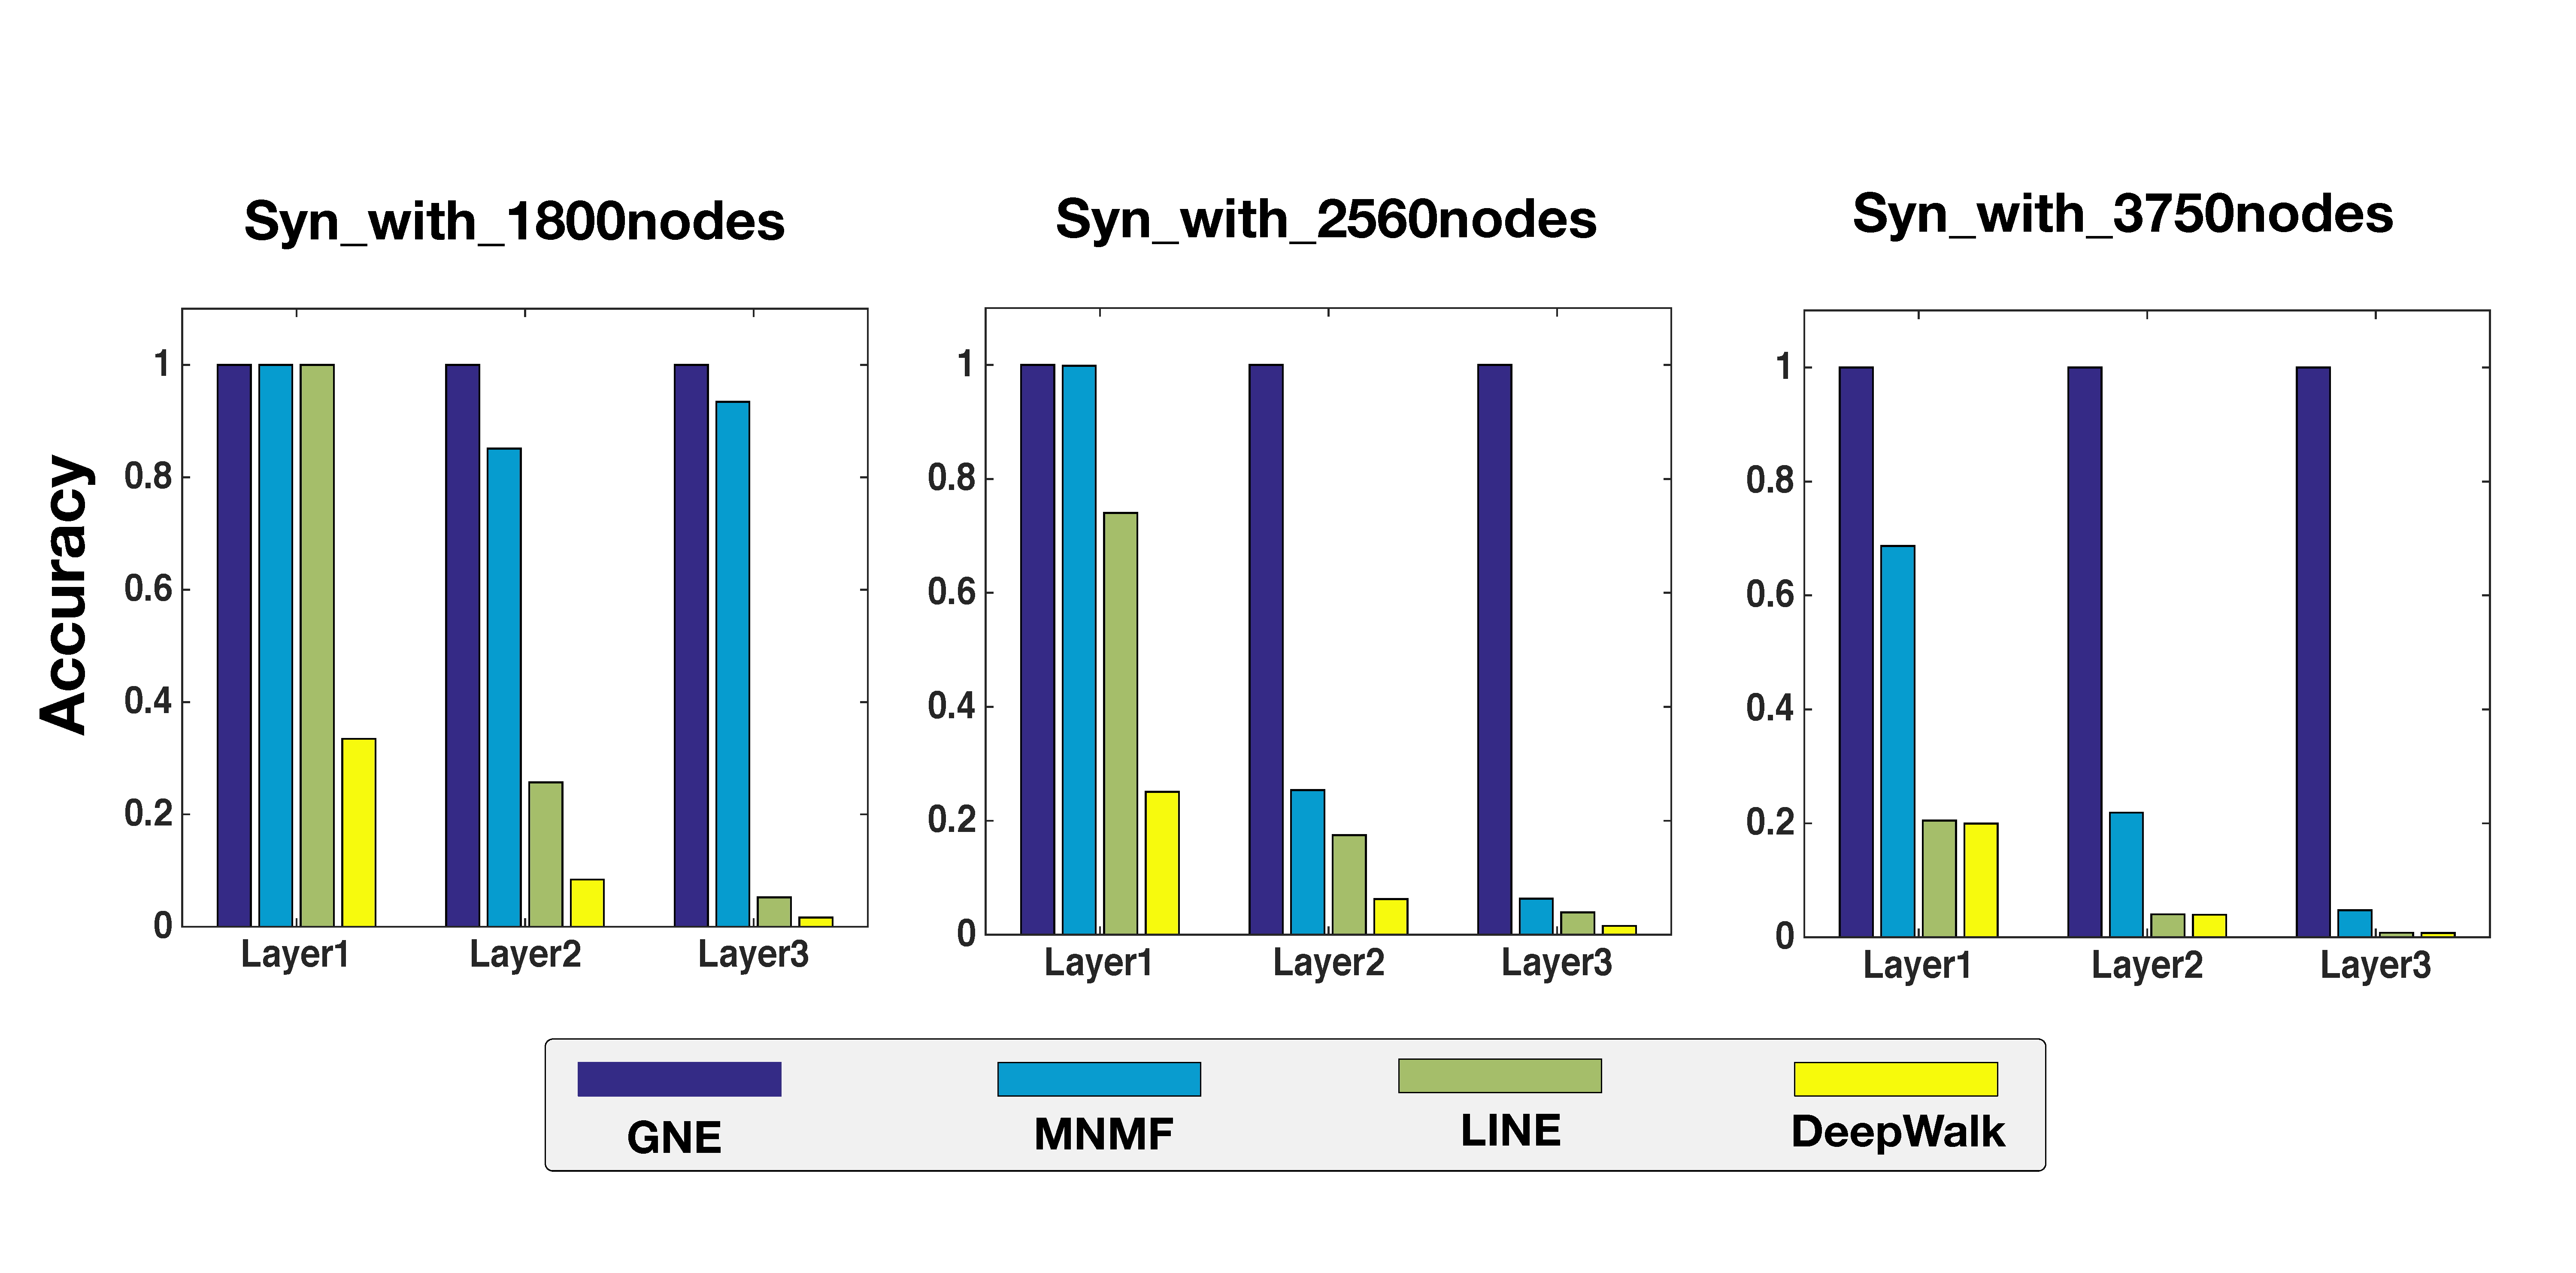
\includegraphics[width=0.8\textwidth]{figure/community_preservation.pdf}
		\caption{The comparision of hierarchical community preservation on different models. Three different structure of HRG but with the same number of layers are used. For each histogram, the horizontal ordinate denotes layer number, and the vertical ordinate denotes the Jaccard's coefficient.}
		\label{fig:community_preservation}
	\end{figure*}

	\begin{figure*}[htb]
		\center
		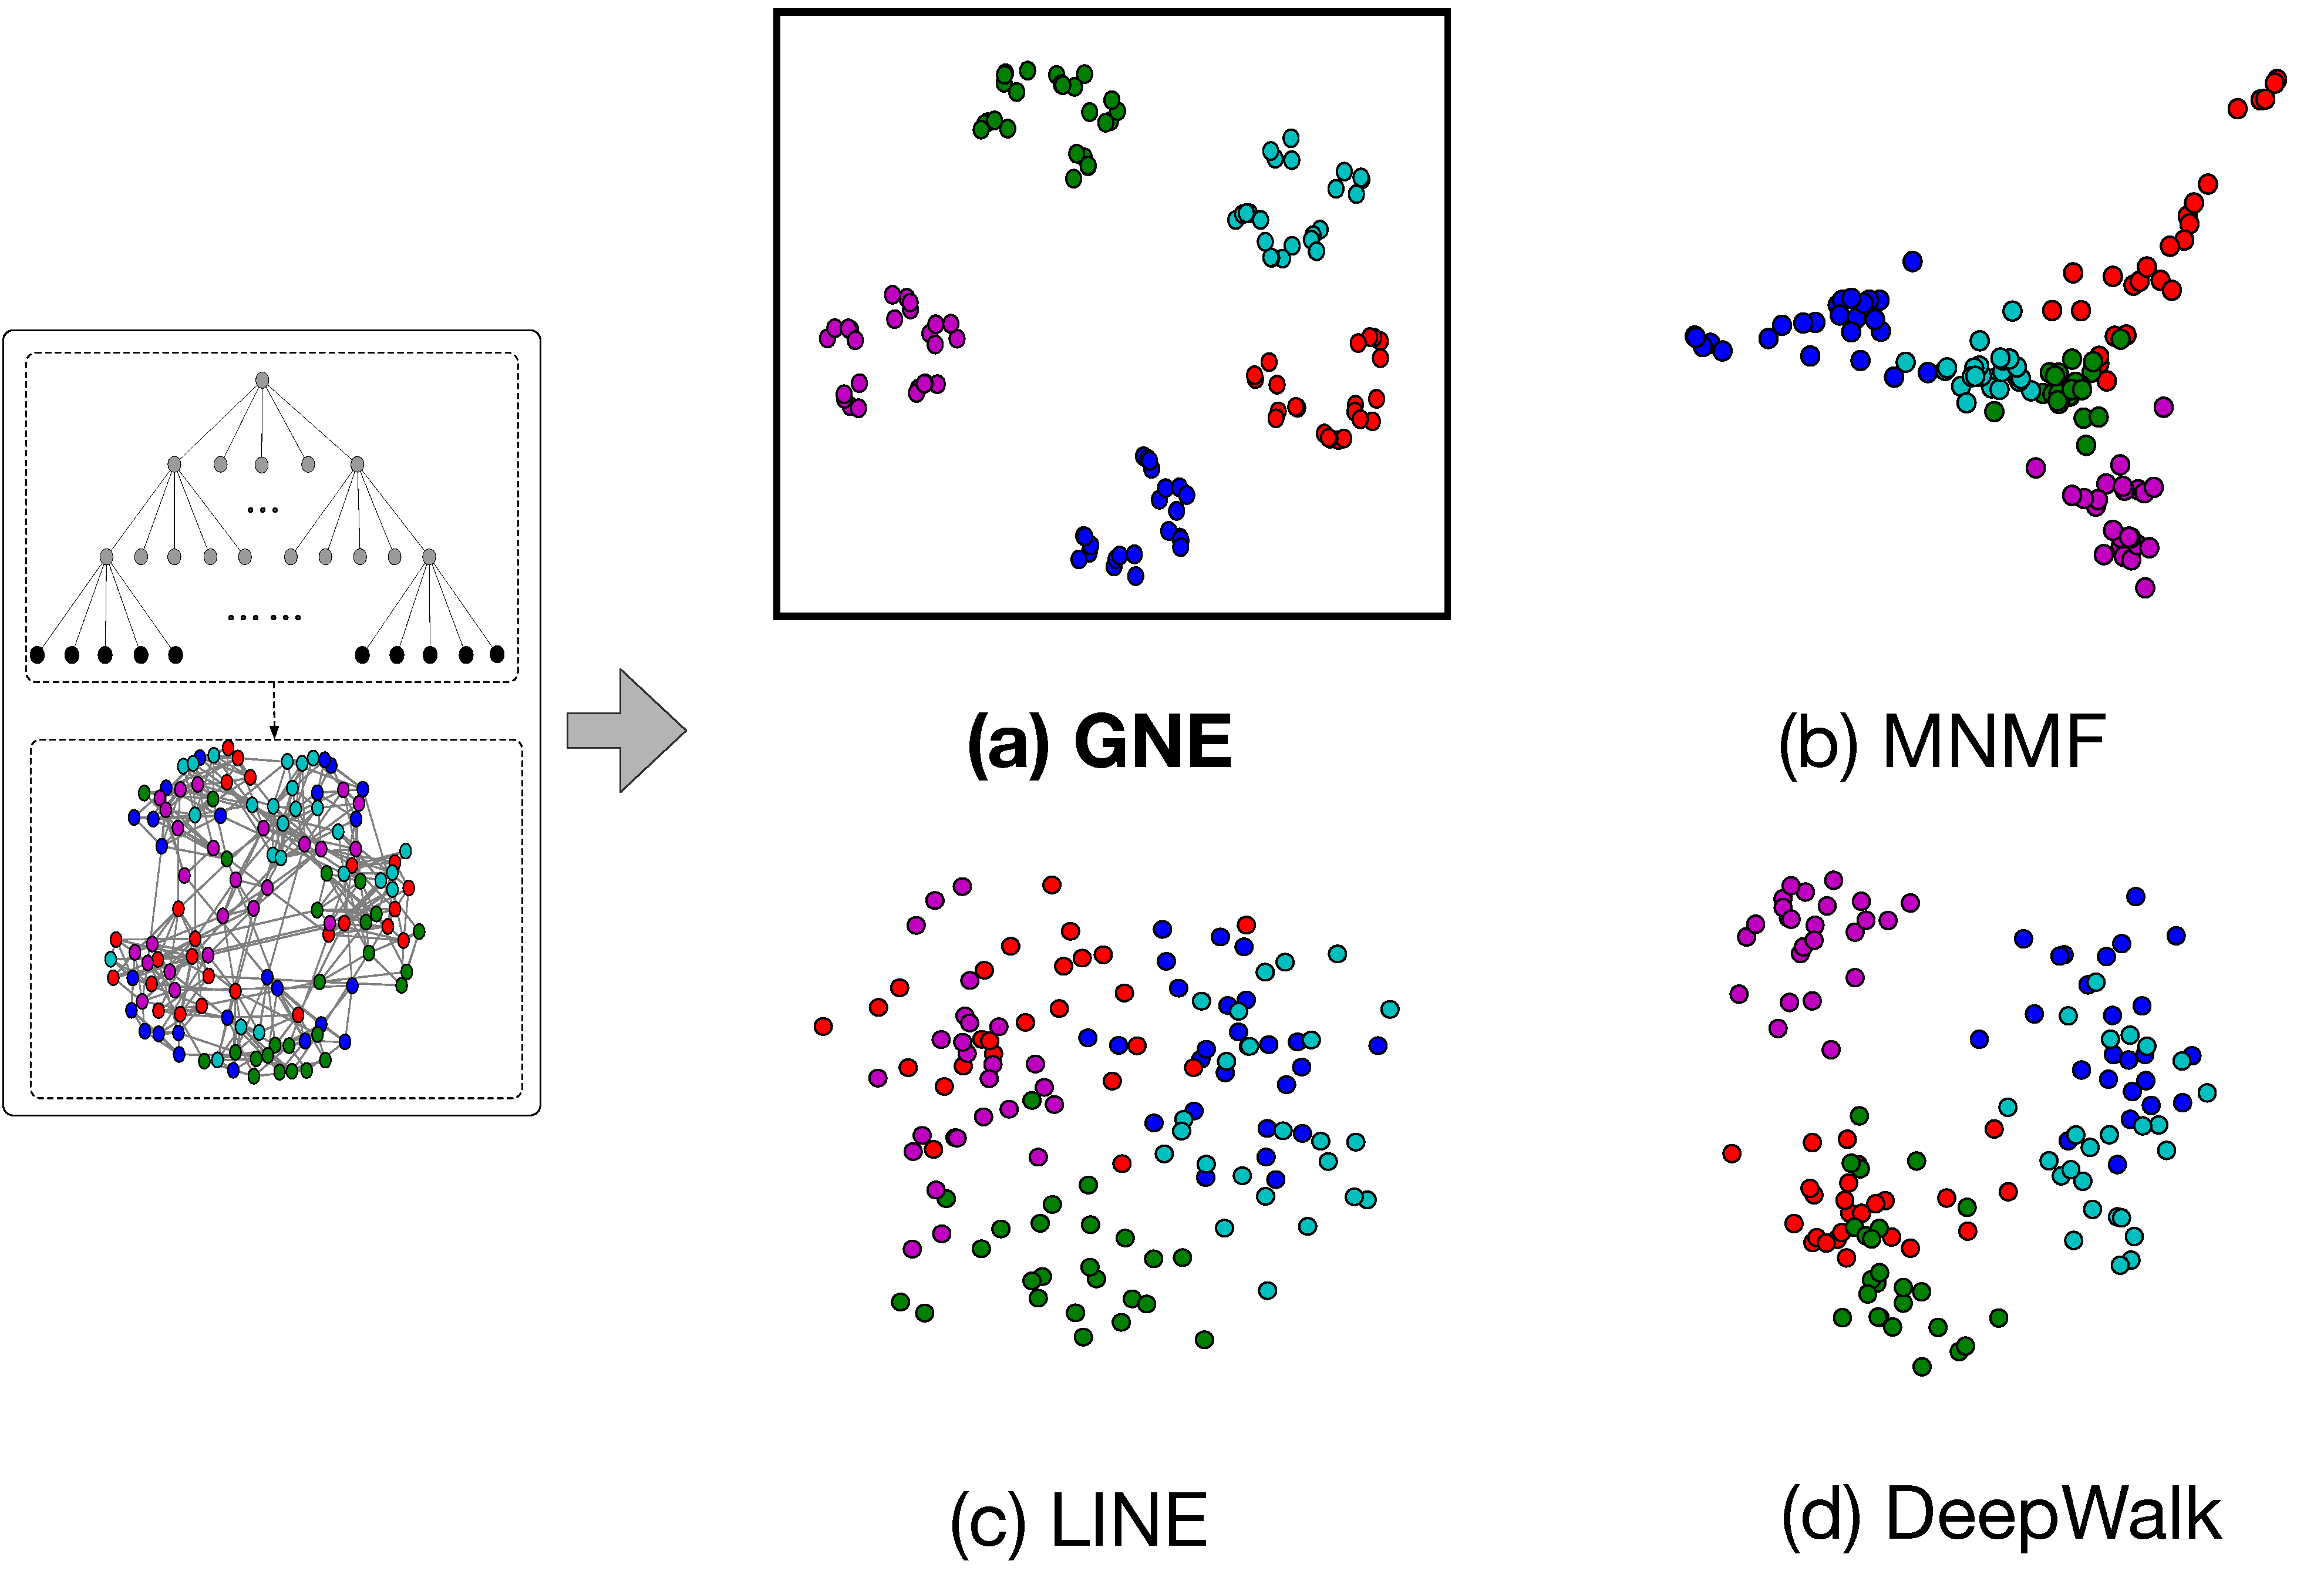
\includegraphics[width=1.0\textwidth]{figure/visualization.pdf}
		\caption{The visualization of node representations on different models}
		\label{fig:visualization}
	\end{figure*}

	

	\begin{table*}[!h]
	  \centering
	  \begin{tabular}{|c|c|c|c|c|c||c|c|c|c|c|}
	   \hline
	   Model& 
	   \multicolumn{5}{c||}{Dolphins} & 
	   \multicolumn{5}{c|}{Polbooks} \\
	   \hline
	   &
	   10\% & 30\% & 50\% & 70\% & 90\% &
	   10\% & 30\% & 50\% & 70\% & 90\%
	   \\
	   \hline
	   GNE & 
	   \textbf{100} & \textbf{100} & \textbf{99.35} & \textbf{97.73} & \textbf{97.14} &
	   \textbf{92.73} & \textbf{88.12} & \textbf{88.11} & \textbf{86.22} &  \textbf{85.89}
	   \\
	   MNMF &
	   78.57 & 73.16 & 67.74 & 68.18 & 67.86 &
	   89.09 & 85.31 & 83.52 & 84.46 & 70.00 
	   \\
	   LINE & 
	   90.00 & 97.37 & 95.16 & 92.27 & 81.96 &
	   82.73 & 80.31 & 81.67 & 79.19 & 72.32
	   \\
	   DeepWalk & 
	   100 & 99.47 & 98.71 & 97.73 & 95.00 &
	   87.27 & 83.44 & 85.56 & 84.19 & 84.42
	   \\
	   \hline
	  \end{tabular}

	  \begin{tabular}{|c|c|c|c|c|c||c|c|c|c|c|}
	   \hline
	   Model& 
	   \multicolumn{5}{c||}{Amherst} & 
	   \multicolumn{5}{c|}{Hamilton} \\
	   \hline
	   &
	   10\% & 30\% & 50\% & 70\% & 90\% &
	   10\% & 30\% & 50\% & 70\% & 90\%
	   \\
	   \hline
	   GNE & 
	   \textbf{94.91} & \textbf{94.25}  &  \textbf{93.94} & \textbf{93.97} & \textbf{93.39} &
	   \textbf{94.66} & \textbf{94.55}  &  \textbf{94.49}  &   \textbf{94.49}  &  \textbf{93.88}
	   \\
	   MNMF &
	   89.82 &  89.06 & 88.04 & 86.43 & 78.44 &
	   91.42 & 90.32 & 89.12 & 87.02 & 81.19
	   \\
	   LINE & 
	   90.76 & 91.82 & 91.48 & 91.09 & 89.42 &
	   92.33 & 92.72 & 92.52 & 92.62 & 91.73
	   \\
	   DeepWalk & 
	   90.62 & 91.65 & 91.32 & 91.13 & 90.41 &
	   92.89 & 92.33 & 92.52 & 92.18 & 91.55
	   \\
	   \hline
	  \end{tabular}

	  \caption{The multi-label classification results on different percentages of test data sets.}
	  \label{tab:classification}
 \end{table*} 

 \begin{table}
		\centering
		\begin{tabular}{|c|c|c|c|}
			\hline
			Name & $|V|$ & $|E|$ & $|Y|$\\
			\hline
			Dolphins & 62 & 159 & 2\\
			%\hline
			Polbooks & 105 & 441 & 3\\
			%\hline
			Hamilton & 2314 & 96394 & 5\\
			%\hline
			Amherst & 2235 & 90954 & 5\\
			\hline
		\end{tabular}
		\caption{Real networks used in experiments. Y denotes the number of classes.}
		\label{tab:real_datasets}
	\end{table}
		
	\begin{table}
		\centering
		\begin{tabular}{|c|c|c|c|}
			\hline
			Name & $|V|$ & $|E|$ & Hierarchy \\
			\hline
			Syn\_with\_125nodes & 125 & 406 & [5,5,5]\\
			Syn\_with\_1800nodes & 1800 & 739637 & [3,4,5,30]\\
			Syn\_with\_2560nodes & 2560 & 1460147 & [4,4,4,40]\\
			Syn\_with\_3750nodes & 3750 & 3066250 & [5,5,5,30]\\
			\hline
		\end{tabular}
		\caption{Hierarchical random networks used in experiments. The hierarchy denotes the number of children per node in each layer, e.g. the tree deriving the HRN with [3,4,5,30] indicates the root node in layer 0 has 3 children, and each node in layer1 has 4 children, and so on.}
		\label{tab:syn_datasets}
	\end{table}


\section{Experiments}
	In this section, we first provide an overview of the datasets and methods which we use in our experiments. Besides, an experimental analysis of our method on both synthetic and real networks is presented. The code of our model is available on Github.
	

	\subsection{Experiment Setup}
	
	\noindent \textbf{Data Sets} 
	An overview of networks we consider in experiments is given in Table \ref{tab:real_datasets} and Table \ref{tab:syn_datasets}. 
	\begin{itemize}
		\item Dolphins data set \cite{lusseau2003bottlenose} is an undirected social network of frequent associations between 62 dolphins in a community living off Doubtful Sound, New Zealand.
		\item Polbooks data set \cite{polbooks} is a network of books about recent US politics sold by the online bookseller Amazon.com. Edges between books represent frequent copurchasing of books by the same buyers.
		\item the Facebook networks \cite{Traud2012Social} comprise 100 colleges and universities. We just choose the social networks in Hamilton University and Amherst College.
	\end{itemize}

	 Besides, in order to evaluate the performance of hierarchical community structure preservation, Hierarchical Random Graphs (HRG) with explicit hierarchical community structure are generated by \cite{clauset2008hierarchical}, of which nodes are originated from the leaves of a tree and edges are derived from the sampling of connected paths between leaves in the tree.

	\noindent \textbf{Relevant Algorithms}
	To validate the performance of our model, we compare it against with state-of-the-art models:
	\begin{itemize}
		\item DeepWalk \cite{Perozzi2014DeepWalk} is to map network into low-dimensional vector spaces by truncated random walks. The sampling strategy in DeepWalk can be seen as a special case of node2vec with $p=1$ and $q=1$.
		\item LINE \cite{Tang2015LINE} is to map network into low-dimensional vector spaces by preserving the first- and second-order proximities of nodes.  
		\item MNMF \cite{Wang2017Community} is to map network into low-dimensional vector spaces by incorporating the community structure into network embedding.
	\end{itemize}

	Additionally, we extract the hierarchical community structure of networks with \cite{Tsvetovat2011Social} as the input of GNE.  

	\subsection{Hierarchical Community Detection}
	In this section, we verify the ability of hierarchical community preservation of our model GNE. We consider synthetic data sets in this experiment, including three different structure of HRG but with the same number of layers(See Table \ref{tab:syn_datasets}). Besides, Jaccard's coefficient \cite{halkidi2001clustering} is applied as an external intex for evaluating the performance of community preservation at each hierarchy of networks.
	
	\begin{equation}
			JC = \frac{|SS|}{|SS|+|SD|+|DS|}
	\end{equation}


	Figure \ref{fig:community_preservation}. shows that the content of the hierarchical community structure can be integrally preserved with our model, no matter how many the number of communities is. However, MNMF preserving community information on a particular resolution is inferior to GNE, and the other model could not perfectly deal with such cases with multi-layer and complex community structure.

	


	\subsection{Network Visualization}
	Network visualization is an important application of network embedding which maps a network into two-dimensional space. We visualize a synthetic network with 125 nodes, 406 edges and 5 communities. Figure \ref{fig:visualization}. presents the visualization experiments. We firstly generate a self-similar network of which nodes are derived from the leaves of five-ary tree with four layers and edges are derived from the sampling of connected paths between leaves in the tree. Additionally, the nodes in the network are classified into different communities with Girvan–Newman algorithm \cite{girvan2002community}. We compare our method against other models.

	For other models, we layout the network into low-dimensional space, and then further map the low-dimensional vectors of the nodes to a 2-D space with t-SNE package \cite{Maaten2008Visualizing}. For our model, we can directly embed network into 2-D vector space according to hyper spherical embedding we proposed.

	It can be seen from Figure \ref{fig:visualization}. that our model GNE embeds nodes on the different-scaled spherical surface hierarchically. It is evident that the node representations of GNE are consistent with modularity property at each hierarchy, i.e. higher intra-cluster similarity but lower inter-cluster similarity. That is to say, GNE integrally preserves the hierarchical community structure. Additionally, GNE has an outstanding performance on clustering nodes compared with others.

	

	\subsection{Multi-label Classification}
	In order to verify the effectiveness of GNE on multi-label node classification, four real social networks with hierarchical community structure are used. The learned representations are used to classify the nodes into a set of labels. Different percentage of nodes are sampled randomly for evaluation, and the rest are for training. The results are averaged over 10 different runs. 

	Table \ref{tab:classification}. shows that GNE has a better performance than other models on different percentage of test data size. Besides, our model is robust no matter how much the percentage of test data accounts for. Specifically, even with 10\% of the samples training, 90\% of the samples testing, the accuracy of our model can still reach 92.57\% on average, 1.98\% higher than DeepWalk, 8.71\% higher than LINE, and 18.20\% higher than MNMF.  
	
	
 
 
 	\section{Conclusion}
 	In this paper, we propose Galaxy Network Embedding (GNE) for network embedding to preserve the hierarchical community structure of a network. 
 	Specifically, we introduce an optimization problem with constraints and transform it into an unconstrained optimization problem more easily to be solved. Besides, we propose a spherical embedding method to maintain the hierarchical community structure from top to down. 
 	Empirically, we verify GNE in a variety of network datasets and applications. The extensive experimental results on vertex clustering and classification, as well as network visualization, demonstrate the advantages of GNE, especially on these networks with hierarchical community structure.
    
\section*{Acknowledgments}

The preparation of these instructions and the \LaTeX{} and Bib\TeX{}
files that implement them was supported by Schlumberger Palo Alto
Research, AT\&T Bell Laboratories, and Morgan Kaufmann Publishers.
Preparation of the Microsoft Word file was supported by IJCAI.  An
early version of this document was created by Shirley Jowell and Peter
F. Patel-Schneider.  It was subsequently modified by Jennifer
Ballentine and Thomas Dean, Bernhard Nebel, and Daniel Pagenstecher.
These instructions are the same as the ones for IJCAI--05, prepared by
Kurt Steinkraus, Massachusetts Institute of Technology, Computer
Science and Artificial Intelligence Lab.

\appendix

\section{\LaTeX{} and Word Style Files}\label{stylefiles}

The \LaTeX{} and Word style files are available on the IJCAI--18
website, {\tt http://www.ijcai-18.org/}.
These style files implement the formatting instructions in this
document.

The \LaTeX{} files are {\tt ijcai18.sty} and {\tt ijcai18.tex}, and
the Bib\TeX{} files are {\tt named.bst} and {\tt ijcai18.bib}. The
\LaTeX{} style file is for version 2e of \LaTeX{}, and the Bib\TeX{}
style file is for version 0.99c of Bib\TeX{} ({\em not} version
0.98i). The {\tt ijcai18.sty} file is the same as the {\tt
ijcai07.sty} file used for IJCAI--07.

The Microsoft Word style file consists of a single file, {\tt
ijcai18.doc}. This template is the same as the one used for
IJCAI--07.

These Microsoft Word and \LaTeX{} files contain the source of the
present document and may serve as a formatting sample.  

Further information on using these styles for the preparation of
papers for IJCAI--18 can be obtained by contacting {\tt
pcchair@ijcai-18.org}.

%% The file named.bst is a bibliography style file for BibTeX 0.99c
\bibliographystyle{named}
\bibliography{GNE}

\end{document}

